\section{Methods}
First some definitions:
By \textit{lattice}, we mean a graph whose nodes are superimposed on a
(potentially infinite) square grid. More precisely, a lattice is a graph whose
nodes are coordinates in 2 dimensional Cartesian space, limited to $\{(x,y) \in
\mathbb{Z} \times \mathbb{Z}\}$, and which may have edges only between nodes
whose euclidean distance is exactly 1.

By \textit{maze} we mean a space of contiguous positions (discrete or not) that 
can be subdivided by walls in any fashion.

The overall method we use for generating mazes can be described as follows:

\begin{enumerate}
	\item We first discover (hopefully) interesting
		grammars, using an evolutionary algorithm.
	\item We create lattices from grammars, each describing the overall
		layout of a maze
	\item We create mazes from lattices. Each node in the lattice
		corresponding to a fixed-size room in the maze, connected to
		other blocks as described by the lattice.
\end{enumerate}

The three steps each involve numerous choices that can be tweaked in accordance
with with the type of maze one wishes to obtain.

\subsection{Evolutionary algorithm}

\subsection{Lattice grammars}
A lattice grammar consists of a set of rules, where a rule is defined by a left-
and a right-hand lattice $(r_p, r_r)$. When a rule $(r_p,r_r)$ is applied to a
lattice, $r_p$ is used as a search pattern in the lattice.
If a match is found, the matching part of the lattice is transformed 
into $r_r$. The lattice is transformed by adding edges that are in $r_r$ but
not in $r_p$, and removing edges that are in $r_p$ but not in $r_r$.

An example of a grammar rule is shown in figure \ref{fig:simplerule}, and an
example of applying that rule to a lattice is shown in figure
\ref{fig:simplerule-applied}. In figure \ref{fig:simplerule-applied}, the rule
has been rotated 90-degrees counter-clockwise to find the match, and the lattice
is transformed accordingly to that rotation. Note that this is not the only
match in the lattice. A different, perhaps more obvious, match exists without
rotation.

\begin{figure}[hbp]
	\centering
	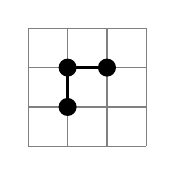
\begin{tikzpicture}
	%grid
	\draw [black!50,step=0.5] (0, 0) grid (1.5, 1.5);

	%nodes
	\foreach \p in {
		(0.5, 0.5),
		(0.5, 1),
		(1.0, 1)
	}\draw [thick, fill=black] \p circle (0.1);

	%paths
	\draw [very thick, color=black] plot coordinates {
		(0.5, 0.5)
		(0.5, 1)
		(1.0, 1)
	};

\end{tikzpicture}
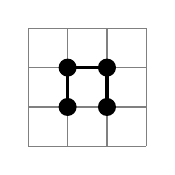
\begin{tikzpicture}
	%grid
	\draw [black!50,step=0.5] (0, 0) grid (1.5, 1.5);

	%nodes
	\foreach \p in {
		(0.5, 0.5),
		(0.5, 1),
		(1.0, 1),
		(1.0, 0.5)
	}\draw [thick, fill=black] \p circle (0.1);

	%paths
	\draw [very thick, color=black] plot coordinates {
		(0.5, 0.5)
		(0.5, 1)
		(1.0, 1)
		(1.0, 0.5)
	};

\end{tikzpicture}

	\caption{The left- and right-hand sides $(r_p,r_r)$ of a lattice-grammar rule that
	adds an edge}
	\label{fig:simplerule}
\end{figure}

\begin{figure}[hbp]
	\centering
	\input{graph-apply-plot.tex}
	\caption{A lattice that is matched by the rule in figure
	\ref{fig:simplerule} (left), and one possible result of applying the
	rule to the lattice (right)}
	\label{fig:simplerule-applied}
\end{figure}

The matching of a rule on a lattice might be implemented without rotation.
Without rotation in the matching process, the choice is deferred to the grammar,
which may or may not include different rotations of a rule. Intuitively,
including rotation in the matching process makes grammars less expressive, but
may help cause self-similarities in the resulting lattice. In practice, the
effect is not entirely obvious, and is tied to the method used to discover
grammars.

Another problem is how a grammar is applied. That is, in
addition to how a single rule is applied, there is the question of how the set
of rules that constitute a grammar is applied. If rules are applied in
succession, the order is significant, as one rule may alter the lattice in a way
that changes how the next rule applies. Of course, this is only true if
application may be done in-place, updating the lattice immediately with each
application. Alternatively, rules could be matched, and then applied together in
a single step. Furthermore, rules may be applied once, or once for each match.
Yet another approach could be to apply each rule repeatedly, continuing to the
next rule only when the first can't be matched to it's own result anymore.

\subsection{Maze generation}
The lattice describes the overall layout of the maze, but by considering the
lattice's nodes as fixed-size rooms, we can decouple the details of the maze layout
from the overall structure. Depending on the room-size, this stage can have
a profound impact on the final result. The connectivity of the maze can be
altered here, and the depth of cul-de-sacs can be decided. In fact, for large
room sizes, cul-de-sacs can be difficult to discern visually on the lattice
level, and may be noticed only at the room level.
